Dieser Abschnitt behandelt Datenzugang und Aufbereitung. Es wird erläutert wie der zum Schätzen der Modelle gebrauchte Datensatz konstruiert wurde und woher die benutzten Prädiktorvarialben kommen. Auch werden Probleme beim beschriebenen Vorgehen angesprochen und mögliche Lösungsansätze vorgeschlagen.

\subsection{Bayern in der Vorgeschichte}
Datenbasis dieser Arbeit sind die Koordinaten archäologischer Fundstellen aus der Vorgeschichte. Peer Fender stellte diesen Datensatz 2016 im Rahmen einer GIS-gestützten Analyse der Siedlungslandschaft Bayerns mit dem Einsatz von Open Data für eine Dissertation zusammen. \cite{fender2017bayern} Dieser Datensatz ist nun für Studenten der LMU unter \cite{Datenbank} frei zugänglich und soll dazu dienen, die Studierenden in die Methoden der Analyse räumlicher Daten mit standard Geoinformationssystemen wie QGIS, SAGA oder GRASS-GIS einzuführen. Die Datenbank enthält über 27000 Einträge von Fundstellen innerhalb Bayerns aus der Bronze-, Eisen- und Späteisenzeit. Natürlich sind nicht nur die Orte an denen Funde gemacht wurden von Interesse, neben Koordinaten im World Geodetic System 1984 (WGS 84) sind Informationen zu Art der Fundstellen wie ``Siedlung'' oder ``Grab'', die Epoche in welche sich die jeweiligen Fundorte einordnen lassen, Höhe über dem Meeresspiegel und viele weitere Kovariablen enthalten. Die weitere Analyse beschränkte sich auf Fundstellen aus der Eisenzeit (Hallstatt- \& La Tènezeit; ca. 800 v. Chr. bis 50 n. Chr.), sowie die folgenden Variablen: 
\begin{itemize}
    \item Höhe über Normalnull
    \item Hangneigung, Hangausrichtung und Topographischer Position Index
    \item Wassernähe 
    \item Durchschnittliche Frosttage pro Jahr
    \item Durchschnittliche Jahrestemperatur
    \item Durchschnittliche Niederschlagsmenge
    \item Durchschnittliche Sonnenstunden pro Tag pro Jahr
\end{itemize}
Diese Variablen wurden ausgewählt, da sie naheliegend zur Modellierung der Habitateignung für eisenzeitliche Menschen erschienen. Klimaeinflüsse wie Temperatur und Niederschlag nehmen Einfluss auf potentielle Nahrungsquellen, Hangneigung und Hangausrichtung und elevationsbaiserte Maße sind von besonderem Interesse, da mit Beginn der Sesshaftigkeit in der Jungsteinzeit auch ein Überblick über ein Siedlungsumfeld relevant für die Wahl eines Niederlassungsortes wurde. \cite{sesshaft} Obwohl das Graben von Brunnen in der Eisenzeit weit verbreitet war, und damit die Nähe zu Gewässern unter Umständen keine Priorität mehr bei der Siedlungswahl darstellte, schien es durchaus sinnvoll zumindest die Distanz zu größeren Gewässern mit in die Analyse einzubeziehen. Siedlungen und Städte sind bis heute vom Trinkwasserzugang und den Transportmöglichkeiten von Gewässern abhängig; außerdem stellte das erzeugen eines Gewässerdistanz-Rasterlayers in R eine interessante Herausforderung dar. \\
Allerdings ergab sich für die weitere Analyse das Problem, dass für etablierte Klassifikationsverfahren wie ein logistisches Modell sowohl Präsenzdaten, also die Ausprägungen der Kovariablen an den Fundstellen, als auch Nonpräsenzdaten, also Werte der interessierenden Variablen an Orten die nicht im Datensatz von Fender enthalten sind, benötigt werden. Eine Möglichkeit dieses Problem zu lösen wäre es, die Daten für Bayern anhand der vorhandenen Messwerte zu interpolieren, und dann an den gewählten Nonpräsenzpunkten die Werte zu messen. Wie in Abbildung \ref{shinyfinal} erkennbar, sind die Sites (Blau) nicht homogen über das gesamte Untersuchungsgebiet verteilt. Dies macht deutlich, dass beispielsweise die Interpolation von Höhen- und Temperaturwerten in Gebirgsnähe nicht mehr trivial zu bewerkstelligen ist, weil sich diese Höhengebiete mit vergleichsweise geringen Temperaturen im Falle Bayerns größtenteils in Grenznähe befinden. Die Mehrheit der Fundstellen (``Sites'') liegt zentraler, im weiten Umfeld der Donau und ihrer Zuflüsse, was bewirkt das für Nonpräsenzpunkte (``Nonsites'') unter großer Ungenauigkeit extrapoliert werden müsste. Das genaue Vorgehen bei der Auswahl von Nonsites wird im Abschnitt zu Pseudo-Nonpresence-Sampling erklärt. \\
Eine bessere Möglichkeit zur Bewältigung des Nonsiteproblems bietet die manuelle Konstruktion eines ``vollständigen'' Datensatzes. Import und Manipulation georeferenzierter Vektor- und Rasterdaten lassen sich in R durch Pakete wie sf \cite{simplefeatures} und raster \cite{raster} mühelos durchführen, was es erlaubt, die Daten von Fender an den gewünschten Positionen zu vervollständigen bzw. einen ``kompletten'' Rasterdatensatz für ganz Bayern zu erstellen und aus diesem benötigte Werte an gewünschten Positionen zu extrahieren. Weil bis auf die minimale Wassernähe alle Variablen von Interesse frei und unkompliziert im Internet verfügbar sind, und weil es sich für spätere Resamplingverfahren und Visualisierungen besser eignet, wurde ein Rasterstack konstruiert aus dem benötigte Messwerte extrahiert wurden. 

\subsection{Rasterdaten}

Um zu gewährleisten, dass alle Rasterlayer die gleichen Ausmaße haben, wurden zunächst die bayrischen Ländergrenzen benötigt. GADM, \cite{GADM.org} eine globale Datenbank administrativer Ländergrenzen eignete sich für diesen Zweck. Die Funktion ``raster::getData'' erlaubt den direkten Import von Vektor- und Rasterdaten aus verschiedenen Datenbanken. In Kombination mit drei Zeichen ISO-Code und der administrativen Ebene (Staat, Bundesland, Landreis etc.) ließ sich so das gewünschte Areal zuschneiden. Eine genaue Erklärung zum Import und der Manipulation von Rasterdaten enthält Kapitel 2 von \cite{lovelace2019}. Im nächsten Schritt wurde ein mit zufälligen Werten vollgeschriebenes Raster erzeugt, welches zum ``masking'' der anderen Daten verwendet wurde. So lassen sich mit den Funktionen ``crop'' und ``mask'' aus dem Raster Paket geographische Daten auf das benötigte Maß zuschneiden. Allgemein wurde für die Konstruktion des Rasterstacks der für die Analyse verwendet wurde nach folgendem Schema verfahren: \\
\begin{enumerate}
    \item Suche nach frei zugänglichen Onlinedaten für gewünschte Variable
    \item Import der Daten in R
    \item Zuschneiden der Daten mit der vorab definierten Maske
    \item Plotten des Rasterlayers um zu prüfen ob Schritte 2 \& 3 erfolgreich waren
\end{enumerate}
Die Höhendaten, das sog. ``Digital Elevation Model'' (DEM) konnten auch via raster::getData importiert werden. Das DEM basiert auf Fernerkundungsdaten die im Jahre 2000 von der Shuttle Radar Topography Mission (SRTM) erhoben wurden. \cite{srtm} Die Auflösung von 90 Metern bildet einen sinnvollen Ansatz für den Rest der Analyse, da die von Fender gesammelten Daten zum größten Teil errechnete Mittelwerte aus einem Radius von 50m um die Fundstellen sind. Für das weitere Vorgehen wurde sich daher an einer Rasterauflösung von 90m pro ``Pixel'' orientiert. \\
Auch Temperatur- und Niederschlagsdaten konnten ähnlich importiert werden. WorldClim Version 2 enthält durchschnittliche monatliche Klimadaten für minimale, mittlere und maximale Temperatur sowie für Niederschlagsmengen der Jahre 1970-2000. \cite{Worldclim2} Aus dieser Datenbank konnten die Daten für Bayern auch via raster::getData importiert werden. \\
Hangneigung, Hangrotation und Topographic Position Index (TPI) mit der in ``raster'' enthaltenen Funktion ``terrain'' aus dem DEM errechnet. Für Neigung und Rotation folgt diese Prozedur dem in \cite{hillshading} beschriebenen Algorithmus basierend auf den Werten der 8 umgebenen Nachbarzellen der Rasterzelle deren Wert errechnet werden soll. TPI ist die Differenz zwischen dem Wert einer Zelle und dem Mittelwert ihrer 8 umgebenden Zellen. Diese Werte können auch, wie in der Dokumentation der Funktion ``terrain'' beschrieben, durch eine focal Operation auf den Rasterdaten errechnet werden. \cite{terraindoku} Sowohl Hangneigung als auch Rotation werden in Grad angegeben. Um die Werte für Hangrotation leichter interpretierbar zu machen wurden diese in einen Faktor mit 8 Ausprägungsstufen konvertiert. Eine Ausprägung von 1 entspricht einer Hangrotation Richtung Norden, eine Ausprägung von 2 Nordosten und so weiter. \\
Die durchschnittliche Anzahl von Frosttagen pro Jahr, sowie die durchschnittliche Anzahl Sonnenstunden pro Tag pro Jahr wurden vom Geoserver des deutschen Wetterdienstes in Form von TIFF Files heruntergeladen und mit der Funktion ``raster::raster'' in Rasterlayer umkonvertiert.\cite{frosttage} \cite{sonnenstunden} In Abbildung \ref{predictorstack} ist das Resultat des Datenimports zu erkennen. Auch in Abbildung \ref{predictorstack} zu sehen, ist der errechnete Rasterlayer, welcher die minimale Entfernung zum nächstgelegenen Gewässer eines jeden Pixels enthält. Wie dieser erzeugt wurde wird im nächsten Abschnitt erläutert. 

\subsection{Gewässer}

Ein sehr mächtiges Werkzeug für Rasterprocessing in R sind die Schnittstellen zu anderen Geoinformationssystemen. Auf Basis von Elevationsdaten lassen sich in GIS allerlei weitere Terraineigenschaften ableiten. So kann über die Schnittstelle zu GRASS GIS mit den Funktionen ``r.stream.extract'' und ``r.stream.distance'' aus einem DEM ein Abflussnetzwerk abgeleitet und im Anschluss daran die Entfernungen von jeder Rasterzelle zu diesem Netzwerk errechnet werden. Leider hatte das DEM aus dem Rasterstack eine zu geringe Auflösung um auf diesem Weg zu sinnvollen Ergebnissen zu kommen. So ließen sich nur die größten Donauzuflüsse und die Donau selbst auf diesem Weg aus dem Höhenmodell errechnen, was als unzureichend eingestuft wurde. \\
Als nächstes wurde versucht eine Funktion zu schreiben, welche für eine beliebige Liste vordefinierter Punkte die minimalen Distanzen zu den in einem Vektordatensatz enthaltenen Flüssen und Gewässern errechnet. Das verwendete Gewässernetz wurde einem online verfügbaren Shapefile entnommen. \cite{rivershapes} Grundidee war hier, die zentralen Koordinaten einer jeden Rasterzelle des Bayernrasters zu entnehmen, die minimalen Distanzen dieser zum Gewässershapefile mit ``geosphere::dist2line'' \cite{dist2line} zu ermitteln und im Anschluss einen Rasterlayer mit allen Distanzen zu rekonstruieren. \\ Obwohl die Ergebnisse vielversprechend aussahen, wurde sich gegen diese Methode entschieden. Grund dafür war unter anderem die hohe Rechenzeit. Selbst nach Parallelisieren dauerte das Errechnen der minimalen Gewässerdistanzen für einzelne Koordinatenpunkte auf der verfügbaren CPU ca. 1.2 Sekunden. Die Gesamtzeit für alle etwa 240000 Rasterzellen hätte also fast 80 Stunden betragen. Natürlich wäre an dieser Stelle ein Profiling der Funktion gekoppelt an das Umschreiben zeitaufwendiger Codeabschnitte in C++ möglich gewesen, dies hätte allerdings den Rahmen der Arbeit gesprengt, da hier in erster Linie Geoprocessing behandelt werden soll. \\
Glücklicherweise lässt sich das am Anfang von Abschnitt 2.2 beschriebene Masking nicht nur zum Zuschnitt von Rasterlayern benutzen. Die für den Brute-Force Ansatz importierten Gewässershapefiles können auch als Maske genutzt werden. Im Anschluss daran können mit der Funktion ``distance'' aus dem raster Paket die minimalen Distanzen zu den Masken für einen ganzen Rasterlayer auf einmal berechnet werden. Als letztes wurden beide so erzeugten Layer für die Entfernungen zum Flussnetzwerk und die Distanzen zu übrigen Gewässern mit der Funktion ``min'' vereint. Da vorimplementierte Rastermethoden deutlich effizienter sind als Werte für einzelne Zellen sequenziell zu bestimmen benötigte diese Vorgehensweise nur etwa 90 Minuten Rechenzeit. \\
Alle Rasterlayer wurden zu einem Rasterstack zusammengefügt. Die Ausprägungen der Variablen für Sites und Nonsites wurden dann mit ``raster::extract'' \cite{extract} aus dem Stack extrahiert. Damit fehlte nur noch ein geeignetes Samplingverfahren für das Ziehen von Nonsitepunkten aus Bayern. Der nächste Abschnitt geht auf diese Problematik ein. 

\subsection{Pseudo-Nonpresence-Sampling}

Das Anwenden von Klassifikationsalgorithmen setzt natürlich eine Einteilung in mindestens zwei verschiedene Klassen voraus. Da der Datensatz von Fender nur Orte enthält an denen Funde gemacht wurden, müssen Nicht-Fundorte also ergänzt werden. Ein in \cite{lovelace2019} beschriebenes Verfahren ist das Ziehen zufälliger Punkte aus dem Forschungsgebiet als ``Pseudo-Nonpräsenzdaten''. Üblicherweise zieht man diese unter der Nebenbedingung, dass sie nicht in eine vordefinierte Bufferzone um die Fundstellen fallen dürfen. Stellt man sich vor, dass Siedlungen im Allgemeinen nicht nur von einzelnen Individuen bewohnt werden und sich der Einflussbereich einer Siedlung nicht auf einen einzigen Punkt konzentriert, macht Bufferzone-Sampling intuitiv Sinn. Allerdings ist die optimale Wahl des Bufferradius nicht trivial. Wird der Radius zu klein gewählt, fallen also die Nonsites unter Umständen zu nah an Sites, so fallen die Ausprägungen beider Klassen aufgrund der räumlichen Korrelation in den Daten sehr ähnlich aus, was zur Folge hat, dass Klassifikationsverfahren überproportional hohe Fehlerraten produzieren. Wird der Radius dagegen zu groß gewählt, so fallen die Ausprägungen beider Klassen überproportional unähnlich aus, was unrealistisch niedrige Fehlerraten zur Folge hätte. Eine weitere Diskussion der Problematik räumlicher Korrelation findet sich in Abscnitt 3.4. Eine Visualisierung des Bufferradiusproblems ist in Abbildung \ref{shinyfinal} zu sehen. \\
Als sinnvoller Mittelweg bot sich ein Bufferradius von 1500 Metern um die Fundstellen an. Nicht nur erlaubt ein ähnlicher Radius moderate False-Positive- \& False-Negative-Rates beim Einschätzen der Modellperformance, auch geht man für die jüngere Eisenzeit in Nordfrankreich davon aus, dass etwa alle 3 km ein Gehöft (ein Einzelhof, einzelnes bebautes Grundstück) lag. \cite{nordfrankreich} Daher wurde davon ausgegangen, dass sich dieser ``Durchmesser'' des Einflussbereiches eisenzeitlicher Siedlungen auch auf andere fruchtbare Gebiete wie das Erdinger Land übertragen lässt. \\
Insgesamt waren nach der Einschränkung auf Fundstellen aus der Eisenzeit und dem Entfernen doppelter Einträge aus dem Datensatz noch 6174 relevante Sites übrig. Für das Schätzen der Modelle wurde die gleiche Menge Nonsites wie hier beschrieben aus Bayern gezogen, also basieren die Resultate auf einem Datensatz mit mehr als 12000 Einträgen. 

\subsection{Visualisierung mit Shiny}

Das Bufferradiusproblem kann innerhalb einer R-Shiny Applikation interaktiv untersucht werden. Zu sehen sind die mit dem Logit-Modell geschätzten predictive maps, die Sites (Blau) sowie die unter der Nebenbedingung des eingestellten Mindestabstandes gezogenen Nonsites in (Rot). Erkennbar wird, dass mit wachsendem Bufferradius die Nonsites in Richtung der Gebirge des Bayrischen Waldes und der Alpen abgedrängt werden. Dies hat zur Folge, dass sich der AUC Wert (Ein Maß für die predictive Performance eines Klassifikators) für wachsenden Bufferradius 1 annähert. Daraus folgt also, dass der gewählte Radius direkten Einfluss auf die Performance der Klassifikatoren nimmt. Auf AUC als Performancemaß für die prädiktive Güte wird in Abschnitt 3.4 näher eingegangen. 
\begin{figure}[H]
    \centering
    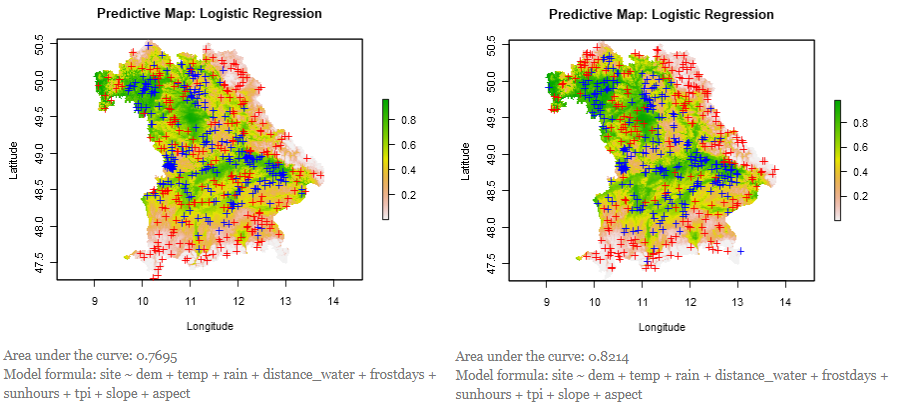
\includegraphics[width = 15cm, height = 7.5cm]{Figures/shinyfinal.png}
    \caption{Visualiserung der Lage von Sites und Nonsites. Links: Bufferradius 1500m. Rechts: Bufferradius 3000m.}
    \label{shinyfinal}
\end{figure}